\section{Experiments}\label{sec:results}

\subsection{Dataset}
The evaluation uses IDD-PeD~\citep{iddped2025}, a pedestrian dataset recorded in unstructured Indian traffic. It contains over 5,000 annotated pedestrians in continuous videos of 45\,s to 10\,min, a median ego speed of 30\,km/h, day and night scenes, per-track behavioural, scene and location annotations, and occlusion labels following the PIE convention. Compared with PIE and JAAD, pedestrians interact with dense traffic without lane discipline and signalisation is often absent, so motion-only trajectory predictors degrade strongly~\citep{iddped2025}. The official protocol uses a 70/30 train/test split, an observation window of 0.5\,s and a prediction horizon of 1.5\,s.

\subsection{Evaluation Metrics and Implementation Details}
All errors are in squared pixels. For predicted boxes $\hat{\mathbf{Y}}$ and ground truth $\mathbf{Y}$ over $H{=}45$ steps, with $\mathbf{c}_t$ the box centre,
\begin{align}
\mathrm{MSE}&=\tfrac1{4H}\textstyle\sum_{t=1}^{H}\|\hat{\mathbf{y}}_t-\mathbf{y}_t\|_2^2,\\
\mathrm{C\text{-}MSE}&=\tfrac1{2H}\textstyle\sum_{t=1}^{H}\|\hat{\mathbf{c}}_t-\mathbf{c}_t\|_2^2,\\
\mathrm{CF\text{-}MSE}&=\tfrac12\|\hat{\mathbf{c}}_H-\mathbf{c}_H\|_2^2,
\end{align}
where C-MSE is the centre MSE over all steps and CF-MSE the centre error at the final step (1.5\,s). The normalisation follows the evaluation routine of the implementation, which is identical for all models.

\paragraph{Matched proof-of-concept protocol.} All models in Table~\ref{tab:unified} use one fixed protocol: a 32/8/24 split of trajectories (training, validation, test), CPU Farneb\"ack optical flow~\citep{farneback2003}, the Adam optimiser with learning rate $10^{-3}$, batch size 8, an MSE loss, \emph{one epoch}, and three random seeds (20260928, 20260929, 20260930). Every tensor with a matching shape is initialised from the official MTN checkpoint. All models therefore see the same data, flow cache and initialisation, and differences can be attributed to the architecture and the seed. The test set consists of 24 held-out trajectories.\verify{number of held-out videos in the unified split} Parameter count and checkpoint size are also reported.

\subsection{Quantitative Results}
Table~\ref{tab:unified} lists the four evaluated models. \CAMTNS obtained the lowest mean MSE, C-MSE and CF-MSE and has the fewest parameters (130,694) and the smallest checkpoint. Relative to \CAMTN, it reduces MSE by $5.0\%$, C-MSE by $4.8\%$ and CF-MSE by $2.8\%$ (Table~\ref{tab:rel}). \DFMTN is worse than \CAMTN on every error metric and has $10.7\%$ more parameters; combining adaptive fusion with encoder self-attention sharing (\DFMTNS) recovers part of the loss on MSE and C-MSE but not on the final-step error.

\begin{table*}[t]
\centering
\caption{Matched comparison of the four models (mean $\pm$ standard deviation over three seeds; squared pixels, lower is better). The best value in each column is in bold.}
\label{tab:unified}
\scriptsize\setlength{\tabcolsep}{3pt}
\resizebox{0.92\textwidth}{!}{\begin{tabular}{p{6.6cm}rrrrr}
\toprule
Model & MSE & C-MSE & CF-MSE & Parameters & Checkpoint (MiB)\\
\midrule
PACE-Net without SATIE (SAGE + MASC) & 1137.11$\pm$20.16 & 1107.40$\pm$19.63 & 2971.36$\pm$103.13 & 139,142 & 1.85\\
PACE-Net (SAGE + MASC + SATIE) (proposed) & \textbf{1080.16$\pm$93.33} & \textbf{1053.83$\pm$95.13} & \textbf{2887.51$\pm$237.14} & \textbf{130,694} & \textbf{1.81}\\
PACE-Net with ROUTE & 1154.78$\pm$9.95 & 1124.20$\pm$10.08 & 3098.16$\pm$137.74 & 154,007 & 1.91\\
PACE-Net with ROUTE and SATIE & 1126.67$\pm$30.84 & 1098.43$\pm$27.25 & 3111.62$\pm$85.57 & 145,559 & 1.88\\
\bottomrule
\end{tabular}
}
\end{table*}

\begin{table}[t]
\centering
\caption{Change relative to \CAMTN, computed from the means of Table~\ref{tab:unified}.}
\label{tab:rel}
\scriptsize\setlength{\tabcolsep}{3pt}
\resizebox{\columnwidth}{!}{\begin{tabular}{p{4.3cm}rrrr}
\toprule
Model (relative to PACE-Net without SATIE (SAGE + MASC)) & $\Delta$MSE & $\Delta$C-MSE & $\Delta$CF-MSE & $\Delta$Params\\
\midrule
PACE-Net (SAGE + MASC + SATIE) & $-$5.01\% & $-$4.84\% & $-$2.82\% & $-$6.07\%\\
PACE-Net with ROUTE & +1.55\% & +1.52\% & +4.27\% & +10.68\%\\
PACE-Net with ROUTE and SATIE & $-$0.92\% & $-$0.81\% & +4.72\% & +4.61\%\\
\bottomrule
\end{tabular}
}
\end{table}

\begin{figure*}[t]
\centering
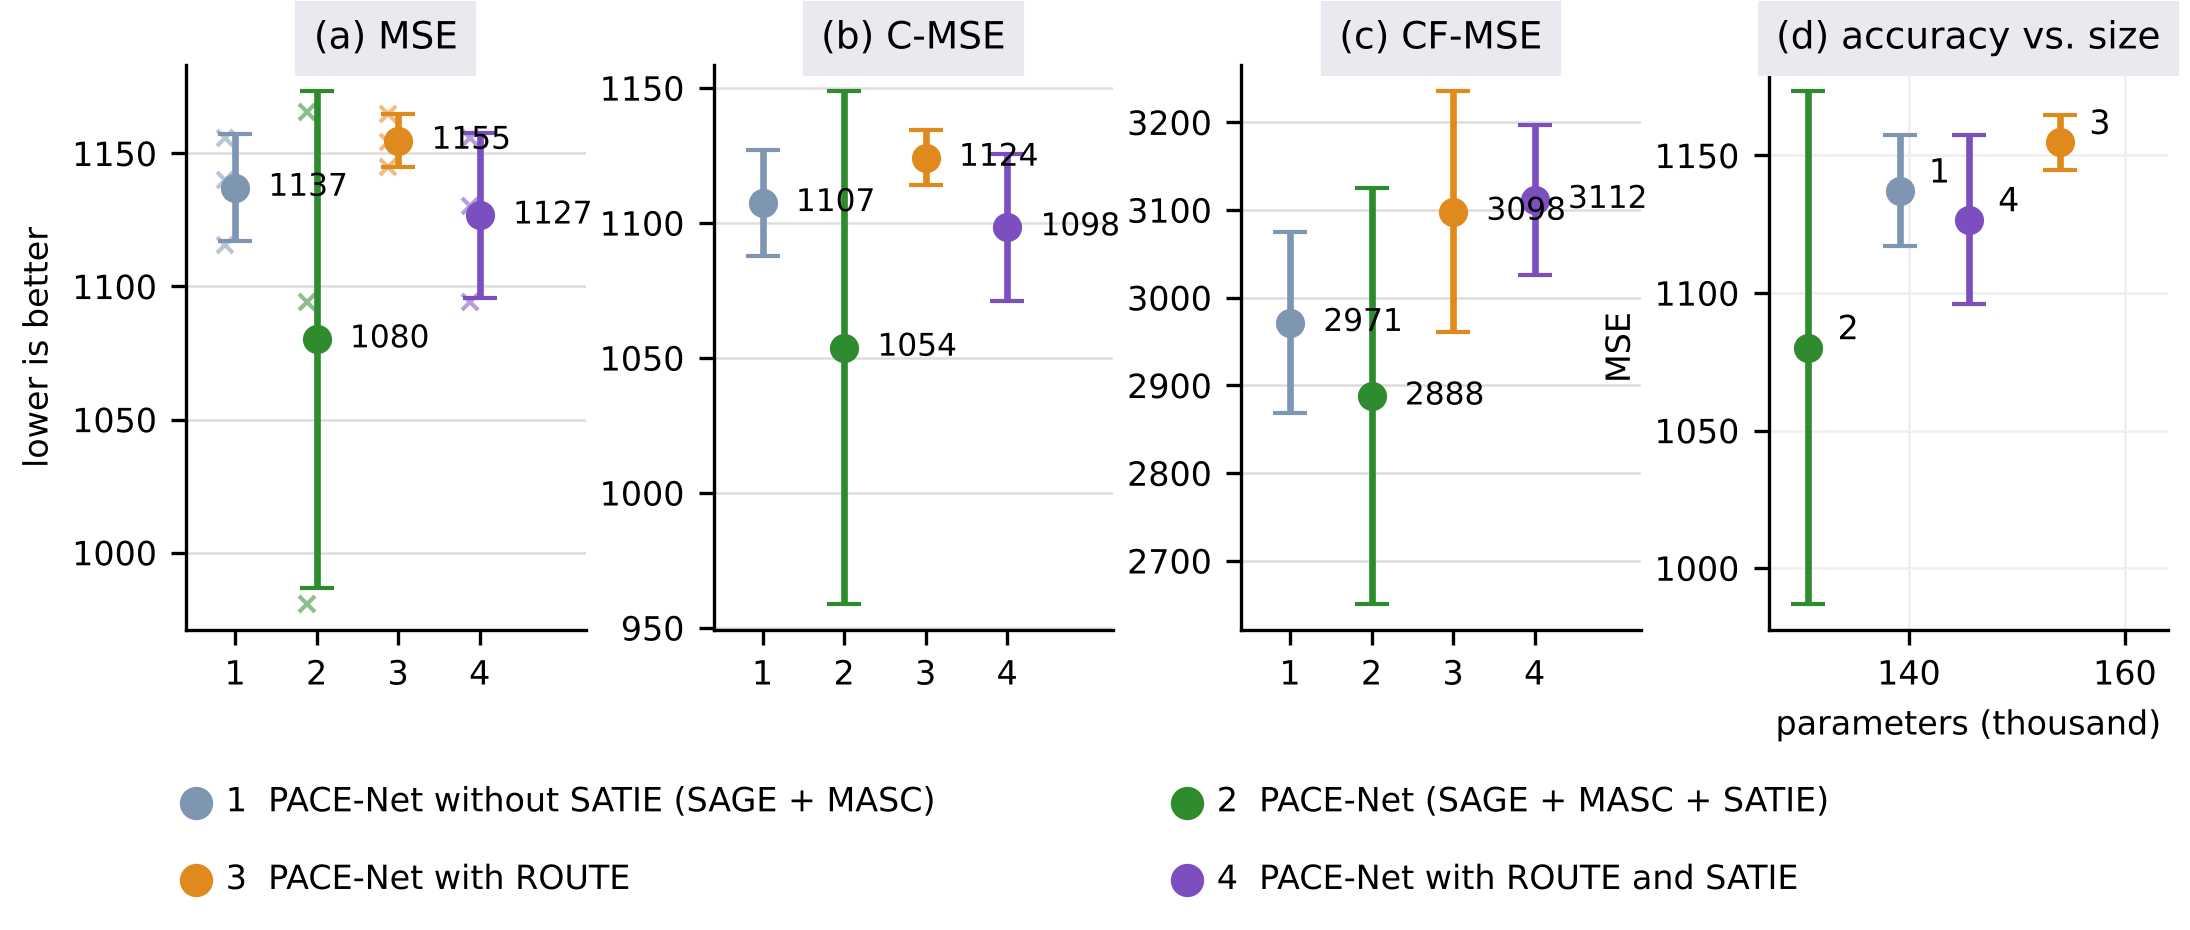
\includegraphics[width=0.92\textwidth]{figures/fig_results.png}
\caption{Test error of the four models. Crosses in panel (a) are individual seeds; dots and bars are mean $\pm$ standard deviation over three seeds. Panel (d) plots MSE against parameter count. Models are numbered as in the legend.}
\label{fig:results}
\end{figure*}

\paragraph{Seed-level behaviour.}
Table~\ref{tab:seed} and Fig.~\ref{fig:seeds} give the per-seed results. \CAMTNS is better than \CAMTN on two of three seeds (by 160 and 61) but worse on the third (by 50), so its standard deviation (93.3) is much larger than that of \CAMTN (20.2). A paired $t$-test over the three seeds gives $p=0.45$; \DFMTN and \DFMTNS are also not significantly different from \CAMTN ($p=0.24$ and $0.73$). The $5\%$ improvement is therefore regarded as a promising but unconfirmed trend. Its practical appeal is that comparable or lower error is obtained with $6\%$ fewer parameters, which is consistent with weight sharing acting as a regulariser in the short, small-data training regime used here.

\begin{table*}[t]
\centering
\caption{Per-seed test MSE and paired statistics against \CAMTN.}
\label{tab:seed}
\scriptsize\setlength{\tabcolsep}{3pt}
\resizebox{0.92\textwidth}{!}{\begin{tabular}{lrrrr}
\toprule
 & \multicolumn{1}{p{2.6cm}}{\raggedleft PACE-Net without SATIE (SAGE + MASC)} & \multicolumn{1}{p{3.4cm}}{\raggedleft PACE-Net (SAGE + MASC + SATIE)} & \multicolumn{1}{p{3cm}}{\raggedleft PACE-Net with ROUTE} & \multicolumn{1}{p{3.6cm}}{\raggedleft PACE-Net with ROUTE and SATIE}\\
Seed & & & &\\
\midrule
20260928 & 1140.10 & 980.57 & 1145.03 & 1094.26\\
20260929 & 1155.60 & 1094.30 & 1164.92 & 1130.09\\
20260930 & 1115.62 & 1165.62 & 1154.39 & 1155.65\\
\midrule
Mean $\pm$ std & 1137.11$\pm$20.16 & 1080.16$\pm$93.33 & 1154.78$\pm$9.95 & 1126.67$\pm$30.84\\
\midrule
Paired $\Delta$ vs.\ PACE-Net without SATIE (SAGE + MASC) (mean $\pm$ sd) & -- & $-$56.95$\pm$104.83 & +17.67$\pm$18.40 & $-$10.44$\pm$44.88\\
Seeds with lower error than PACE-Net without SATIE (SAGE + MASC) & -- & 2/3 & 0/3 & 2/3\\
Paired $t$-test $p$-value ($n{=}3$) & -- & 0.45 & 0.24 & 0.73\\
\bottomrule
\end{tabular}
}
\end{table*}

\begin{figure}[t]
\centering
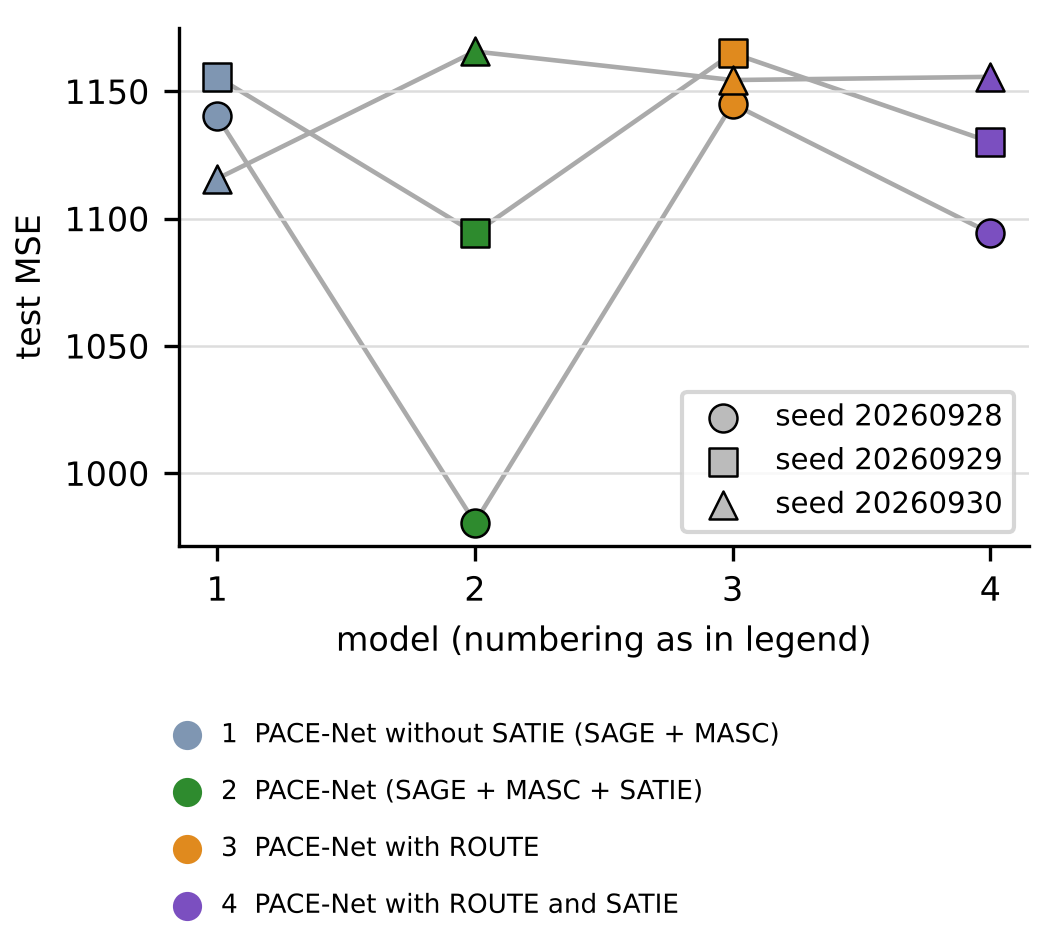
\includegraphics[width=\columnwidth]{figures/fig_seeds.png}
\caption{Per-seed test MSE of the four models; lines connect results obtained with the same seed. Models are numbered as in the legend.}
\label{fig:seeds}
\end{figure}

\paragraph{Computational cost.}
Encoder self-attention sharing reduces the number of unique parameters and the checkpoint size but not the amount of computation, since the three self-attention operations are still executed. The adaptive-fusion models evaluate all three fusion candidates before selecting one and are therefore both larger and no cheaper. Inference-time results are not reported, because timing on a shared CPU was too noisy to support a conclusion.

\paragraph{Effect of scene context.}
In an earlier single-seed study (12 epochs, 10 held-out trajectories of one video, the same CPU flow), adding the gated context token reduced MSE from 1242.98 to 1113.21 ($-10.4\%$), C-MSE from 1225.17 to 1094.57 and CF-MSE from 4093.85 to 3646.51 ($-10.9\%$). Because the protocol differs from Table~\ref{tab:unified} (training length, test set, number of seeds), these values are not directly comparable with it; re-running the baseline in the matched protocol is part of the planned work (Sec.~\ref{sec:limits}).

\subsection{Comparison with Prior Work}
Table~\ref{tab:prior} places the present results next to the published IDD-PeD trajectory benchmarks~\citep{iddped2025}: the deterministic PIETraj~\citep{rasouli2019pie} and MTN~\citep{yin2021mtn} and the stochastic BiTraP~\citep{yao2021bitrap} and SGNet~\citep{wang2022sgnet}, which report the best of 20 samples.

\begin{table}[t]
\centering
\caption{Comparison with published results (MSE, C-MSE, CF-MSE at 1.5\,s, squared pixels). Published rows are copied from Table~III of~\citep{iddped2025} (full test split, RAFT flow, GPU training). The rows for the present models use the reduced protocol described above and are therefore \emph{not directly comparable}.}
\label{tab:prior}
\scriptsize\resizebox{\columnwidth}{!}{%
\begin{tabular}{p{4.7cm}lrrr}
\toprule
Method & Type & MSE & C-MSE & CF-MSE\\
\midrule
PIETraj~\citep{rasouli2019pie} & deterministic & 2181 & 1979 & 8960\\
MTN~\citep{yin2021mtn} & deterministic & 1652 & 1489 & 6668\\
BiTraP~\citep{yao2021bitrap} & stochastic (best of 20) & 338 & 200 & 638\\
SGNet~\citep{wang2022sgnet} & stochastic (best of 20) & 310 & 190 & 531\\
\midrule
MTN, early single-seed study & deterministic & 1243 & 1225 & 4094\\
\CAMTN, early single-seed study & deterministic & 1113 & 1095 & 3647\\
\CAMTN, matched protocol & deterministic & 1137 & 1107 & 2971\\
\CAMTNS, matched protocol (proposed) & deterministic & 1080 & 1054 & 2888\\
\bottomrule
\end{tabular}}
\end{table}

\paragraph{Discussion.} Among deterministic methods, the published MTN reaches an MSE of 1652 on the official benchmark and PIETraj 2181; the context-aware models of this paper obtain 1080--1137 in the reduced protocol, which is in the same range as or below MTN, and the context token lowers the error relative to the motion-only baseline of the early study. The stochastic BiTraP and SGNet are about $3.5$--$5\times$ lower in MSE, as expected, because they report the best of 20 sampled futures and are goal-conditioned, whereas the proposed model outputs a single trajectory; closing this gap would require a multimodal output head, which is beyond the scope of this work. \textbf{These comparisons are indicative only}: the present numbers come from 24 trajectories, one training epoch and Farneb\"ack flow, whereas the published numbers use the entire 30\% test split, RAFT flow~\citep{teed2020raft} and fully trained GPU models. A fair claim of improvement over MTN requires re-running the baseline under exactly the same conditions as the proposed model, as described in Sec.~\ref{sec:ablation}.
